\documentclass[a4paper,12pt]{article}
\usepackage[utf8]{inputenc}
\usepackage[german]{babel}
\usepackage{amsmath}
\usepackage{amssymb}
\usepackage{amsthm}
\usepackage{geometry}
\usepackage{graphicx}
\usepackage{tikz}
\usetikzlibrary{arrows,positioning,shapes}
\usepackage[hidelinks]{hyperref}

\geometry{margin=2.5cm}

\theoremstyle{definition}
\newtheorem{definition}{Definition}
\newtheorem{beispiel}{Beispiel}
\newtheorem{satz}{Satz}

\title{Zufall in der Mathematik}
\author{Stephan Epp}
\date{\today}

\begin{document}
	
\maketitle

\tableofcontents
\newpage

\section{Einführung}

Zufall wird in der Mathematik beschrieben für diskrete und kontinuierliche Ereignisse. Diskrete Ereignisse sind dabei die natürlichen Ereignisse, die sich jeder gut vorstellen kann. Ein diskretes Ereignis ist zum Beispiel das Würfeln eines Würfels. Ein Würfel hat sechs Seiten. Dabei hat jeden Seite des Würfels eine Augenzahl, dass jede Augenzahl von $1, \ldots, 6$ auf jeweils einer Würfelseite abgebildet ist. Es stellt sich die Frage, wenn jemand den Würfel einmal würfelt, auf welche Augenzahl der Würfel fällt? Da es sechs Seiten gibt, kann es sein, dass der Würfel bei einem Wurf zufällig auf die Augenzahl $3$ fällt. Ist die $3$ auf dem Würfel deshalb bevorzugt, weil der Würfel beim Wurf auf die Augenzahl $3$ gefallen ist? Kommt es zufällig öfter vor, dass der Würfel auf die Augenzahl $3$ fällt? Nein, der Würfel hat sechs gleich große Seiten und keine der Seiten des Würfels ist durch die Art des Würfels bevorzugt.

\section{Grundlagen}

Um jede Unruhe über den Ausgang des Zufalls allen Beteiligten zu nehmen, wird der Zufall für diskrete Ereignisse mit Hilfe der Mathematik beschrieben und analysiert. 

\subsection{Definitionen}

Für das diskrete Ereignis, bei dem ein Würfel einmal geworfen wird, können folgende diskrete Ereignisse zufällig eintreten. Der Würfel kann auf die Augenzahl $1$ fallen, der Würfel kann auf die Augenzahl $2$ fallen, ..., der Würfel kann auf die Augenzahl $6$ fallen. Dabei ist jeder Fall des Würfels auf eine andere Augenzahl ein Ereignis. Es gibt damit also sechs Ereignisse beim Würfeln des Würfels mit sechs Seiten.  

Ein \textit{Versuch} beschreibt das Vorhaben zum Beispiel einen Würfel zu würfeln. In diesem Versuch können unterschiedliche Ereignisse zufällig eintreten. \textit{Die Menge aller Ereignisse für einen Versuch}, die zufällig eintreten können, wird definiert mit $\Omega$. Um nun zu sagen, wie zufällig es ist, dass der Würfel beim Wurf auf die Augenzahl $3$ fällt, muss nur dieses Ereignis ins Verhältnis zu allen möglichen Ereignissen gesetzt werden. Damit ergibt sich als Wert für den Zufall des Ereignisses, dass der Würfel beim Wurf auf die Augenzahl $3$ fällt, die \textit{Wahrscheinlichkeit} von $\frac{1}{6}$. Es fällt auf, dass für jedes Ereignis dieses Versuches gilt, dass der Würfel beim Wurf auf die Augenzahl $k$ fällt, die \textit{Wahrscheinlichkeit} $\frac{1}{6}$ hat, $k \in \Omega = \{1, \ldots, 6\}$. Denn der Würfel hat ja sechs gleich große Seiten und keine der Seiten des Würfels ist durch die Art des Würfels bevorzugt. Ist die Summe aller Wahrscheinlichkeiten der Zufälle aller Ereignisse insgesamt $1$, wurden alle Ereignisse des Versuchs berücksichtigt und der Versuch ist \textit{mathematisch vollständig beschrieben}.

Für Versuche, die durch diskrete Ereignisse beschrieben werden, ist die Überprüfung der vollständigen mathematischen Beschreibung notwendig. Erst dann liegt eine mathematische Beschreibung vor, auf deren Grundlage weitere Ereignisse für diesen Versuch betrachtet und analysiert werden können. Für den Versuch einen Würfel einmal zu würfeln kann man sich auch fragen, wie wahrscheinlich der Zufall für das Ereignis ist, dass der Würfel nicht auf den Augenzahl $3$ fällt. Das ist komplizierter, im Allgemeinen. Glücklicherweise aber betrachten wir diskrete Ereignisse. Deshalb lässt sich die Wahrscheinlichkeit für den Zufall des Ereignisses, dass der Würfel nicht auf die Augenzahl $3$ fällt, wie folgt \textit{abzählen}. Die Wahrscheinlichkeit für den Zufall des Ereignisses, dass der Würfel nicht auf die Augenzahl $3$ fällt, ist dieselbe für den Zufall der Ereignisse, dass der Würfel auf die Augenzahl $1, 2, 4, 5$ oder $6$ fällt. Dies sind fünf Ereignisse. Damit ergibt sich eine Wahrscheinlichkeit für den Zufall des Ereignisses, dass der Würfel nicht auf die Augenzahl $3$ fällt, von $\frac{5}{6}$.

\subsection{Zufallsvariable}

Für Versuche, die durch diskrete Ereignisse beschrieben werden, ist es für die Analyse manchmal hilfreich, eine Zufallsvariable zu verwenden. Dabei beschreibt die Zufallsvariable den Zufall für das Ereignis variabel für den konkreten Ausgang. Zum Beispiel kann für den Versuch, einen Würfel zu würfeln, eine Zufallsvariable definiert werden durch 
\begin{align}
	\label{math:var-x}
	X = \{\text{Anzahl der Augen, auf die der Würfel fällt}\}.
\end{align}

Es fiel auf, dass für jedes Ereignis dieses Versuches gilt, dass der Würfel beim Wurf auf die Augenzahl $k$ fällt, die \textit{Wahrscheinlichkeit} $\frac{1}{6}$ hat, $k \in \{1, \ldots, 6\}$. Mit der Zufallsvariable ist diese Beobachtung nun so beschreibbar $P(X = k) = \frac{1}{6}$, wobei $P$ für Probability steht.

\subsection{Erwartungswert}

Bei dem Versuch, den Würfel zu würfeln, ist es vor dem Versuch von Bedeutung, zu ermitteln, welcher Ausgang des Versuches zu erwarten ist. Für Versuche, die durch diskrete Ereignisse beschrieben werden, wird der Erwartungswert $E$ für eine Zufallsvariable $X$ so berechnet:
\begin{align}
	E[X] &= \sum_{k \in \Omega} k \cdot P(X = k).
\end{align}
Für die Zufallsvariable $X$ von (\ref{math:var-x}) ergibt sich damit ein Erwartungswert von
\begin{align}
	E[X] &= \sum_{k \in \{1, \ldots, 6\}} k \cdot P(X = k) \\
		 &= 1 \cdot P(X = 1) + \ldots + 6 \cdot P(X = 6) \\
		 &= 1 \cdot \frac{1}{6} + \ldots + 6 \cdot \frac{1}{6} \\
		 &= 3,5.
\end{align}
Das bedeutet, bevor wir den Würfel einmal gewürfelt haben, erwarten wir, dass der Würfel auf die Augenzahl 3,5 fällt. Diese Augenzahl gibt es nicht. Der Erwartungswert aber beschreibt formal am genauesten, welcher Ausgang bei diesem Versuch wirklich zu erwarten ist. Denn erst wenn wir diesen Versuch oft wiederholen, ist es interessant, wie der tatsächliche Ausgang des Versuches vom Erwartungswert abweicht.

\subsection{Bedingte Wahrscheinlichkeit}
Die bedingte Wahrscheinlichkeit geht auf Arbeiten von \textsc{Pierre-Simon Laplace} und auf \textsc{Andrej N. Kolmogorow} zurück. Seien $A$ und $B$ zwei Ereignisse mit $P(B) > 0$, dann beschreibt die bedingte Wahrscheinlichkeit $P(A \mid B)$ die Wahrscheinlichkeit des Ereignisses $A$ unter der Voraussetzung, dass das Ereignis $B$ bereits eingetreten ist. Formal wird die \textit{bedingte Wahrscheinlichkeit} definiert durch

\begin{align}
P(A \mid B) = \frac{P(A \cap B)}{P(B)}.
\end{align}
Aus der Definition folgt unmittelbar die \emph{Produktregel}

\begin{align}
P(A \cap B) = P(A \mid B)\cdot P(B),
\end{align}
welche eine wichtige Rolle in der Wahrscheinlichkeitsrechnung hat. Eine Besonderheit ergibt sich im Fall der Unabhängigkeit zweier Ereignisse. Die \textit{Unabhängigkeit} von $A$ und $B$ ist definiert durch
\begin{align}
P(A \cap B) = P(A)\cdot P(B).
\end{align}
Setzt man diese Beziehung in die Definition der bedingten Wahrscheinlichkeit ein, so erhält man
\begin{align}
P(A \mid B) = \frac{P(A)\cdot P(B)}{P(B)} = P(A),
\end{align}
was zeigt, dass das Eintreten von $B$ keinen Einfluss auf die Wahrscheinlichkeit von $A$ hat. Dieses Ergebnis war zu erwarten, denn wenn $A$ und $B$ unabhängige Ereignisse sind, also $A \cap B = \emptyset$, dann kann $B$ keinen Einfluss haben auf $P(A \mid B)$, also $P(A \mid B) = P(A)$. Warum die formale Definition der bedingten Wahrscheinlichkeit (7) auch Sinn macht, ist die Beobachtung, dass für $P(A \mid B)$ folgendes bestimmt werden soll. Unter der Voraussetzung, dass $B$ gilt, ist die Wahrscheinlichkeit von $A$ zu bestimmen und $A$ und $B$ sind abhängig, das heißt $A \cap B \neq \emptyset$. Es ist $B$ als die Menge aller Ereignisse zu wählen, da nach der konkreten Wahrscheinlichkeit von $A$ gefragt wird unter der Voraussetzung, dass $B$ gilt, das heißt $P(A \cap B) / P(B)$.

\section{Markov-Ketten}

Die Konzepte der bedingten Wahrscheinlichkeit und der Unabhängigkeit finden eine wichtige Anwendung in der Modellierung von Markov-Ketten. Eine Markov-Kette beschreibt einen Versuch, bei dem das System verschiedene Zustände durchlaufen kann. Der entscheidende Aspekt einer Markov-Kette ist die \textit{Gedächtnislosigkeit} oder \textit{Markov-Eigenschaft}. Diese besagt, dass die Wahrscheinlichkeit für den Übergang in den nächsten Zustand nur vom aktuellen Zustand abhängt und unabhängig ist von der gesamten Vorgeschichte des Systems. Dies ist eine besondere Form der Unabhängigkeit.

\begin{definition}[Markov-Kette]
	Eine zeitdiskrete Markov-Kette ist ein stochastischer Prozess $(X_t)_{t \geq 0}$ mit endlichem Zustandsraum $S = \{s_1, s_2, \ldots, s_n\}$ und der Markov-Eigenschaft:
	\begin{align}
		P(X_{t+1} = s_j \mid X_t = s_i, X_{t-1}, \ldots, X_0) = P(X_{t+1} = s_j \mid X_t = s_i) = p_{ij}
	\end{align}
	wobei $p_{ij}$ die Übergangswahrscheinlichkeit von Zustand $s_i$ nach $s_j$ ist.
\end{definition}

Die Markov-Eigenschaft bedeutet also, dass der zukünftige Zustand $X_{t+1}$ unabhängig ist von allen vergangenen Zuständen $X_{t-1}, X_{t-2}, \ldots, X_0$, gegeben den aktuellen Zustand $X_t$. Diese bedingte Unabhängigkeit ist der Kern der Markov-Eigenschaft. Die Wahrscheinlichkeit $P(X_{t+1} = s_j \mid X_t = s_i)$ wird hier als Notation verwendet, um auszudrücken, dass das System sich im Zustand $s_i$ befindet. Die entscheidende Eigenschaft ist aber, dass diese Wahrscheinlichkeit vollständig durch $p_{ij}$ beschrieben wird und unabhängig davon ist, wie das System in den Zustand $s_i$ gelangt ist. Alle Übergangswahrscheinlichkeiten werden in der \textit{Übergangsmatrix} zusammengefasst.

\begin{definition}[Übergangsmatrix]
	Die Übergangsmatrix $P = (p_{ij})$ einer Markov-Kette ist eine stochastische Matrix mit:
	\begin{align}
		p_{ij} \geq 0 \quad \text{und} \quad \sum_{j=1}^{n} p_{ij} = 1 \quad \text{für alle } i
	\end{align}
\end{definition}

Die Bedingung $\sum_{j=1}^{n} p_{ij} = 1$ für alle $i$ ist notwendig, denn von jedem Zustand aus muss das System in irgendeinen Zustand übergehen, möglicherweise auch in denselben Zustand bleiben. Damit ist der Versuch für jeden Zustand mathematisch vollständig beschrieben.

Die Gedächtnislosigkeit vereinfacht die Analyse von Markov-Ketten erheblich. Anstatt die gesamte Historie des Systems zu berücksichtigen, genügt es, nur den aktuellen Zustand zu kennen. Dies ist eine massive Reduktion der Komplexität. Wenn mehrere Schritte betrachtet werden, kann die Wahrscheinlichkeit für Übergänge über mehrere Zeitschritte durch wiederholte Anwendung der Produktregel berechnet werden. Die Wahrscheinlichkeit, dass das System nach zwei Schritten von Zustand $s_i$ nach Zustand $s_k$ übergeht, berechnet sich durch Summation über alle möglichen Zwischenzustände:
\begin{align}
	P(X_{t+2} = s_k \mid X_t = s_i) = \sum_{j=1}^{n} P(X_{t+2} = s_k \mid X_{t+1} = s_j) \cdot P(X_{t+1} = s_j \mid X_t = s_i).
\end{align}
Dies bedeutet, dass über alle möglichen Zwischenzustände $s_j$ summiert wird. Für jeden Zwischenzustand wird die Wahrscheinlichkeit berechnet, von $s_i$ nach $s_j$ zu gelangen und von dort nach $s_k$. Die Summe aller dieser Pfade ergibt die Gesamtwahrscheinlichkeit für den Übergang von $s_i$ nach $s_k$ in zwei Schritten. Mit der Übergangsmatrix $P$ lässt sich dies kompakt schreiben als
\begin{align}
	P(X_{t+2} = s_k \mid X_t = s_i) = (P^2)_{ik},
\end{align}
wobei $P^2$ das Matrixprodukt $P \cdot P$ ist. Allgemein gilt für $n$ Schritte
\begin{align}
	P(X_{t+n} = s_k \mid X_t = s_i) = (P^n)_{ik}.
\end{align}
Die Wahrscheinlichkeit für Übergänge über mehrere Schritte ergibt sich damit direkt aus der Potenzierung der Übergangsmatrix. Dies ist eine elegante Konsequenz der Gedächtnis\-losigkeit.

\begin{beispiel}
Ein verteiltes Softwaresystem zur Verwaltung von Kundendaten besteht aus mehreren Komponenten, die unterschiedliche Funktionen bereitstellen. Das System kann sich in verschiedenen Zuständen befinden, die die Anzahl der aktiven Komponenten beschreiben. Die Zustände sind: $s_1$ (alle 12 Komponenten aktiv), $s_2$ (11 Komponenten aktiv), $s_3$ (10 Komponenten aktiv), $s_4$ (9 Komponenten aktiv), $s_5$ (8 Komponenten aktiv), $s_6$ (7 Komponenten aktiv), $s_7$ (6 Komponenten aktiv), $s_8$ (5 Komponenten aktiv), $s_9$ (4 Komponenten aktiv), $s_{10}$ (3 Komponenten aktiv), $s_{11}$ (2 Komponenten aktiv - degradiert), $s_{12}$ (1 Komponente aktiv - kritisch). Im Zustand $s_1$ arbeitet das System mit voller Leistung. Die Zustände $s_2$ bis $s_{10}$ beschreiben schrittweise Reduktionen der verfügbaren Komponenten, wobei das System weiterhin stabil arbeitet. Der Zustand $s_{11}$ ist degradiert, denn mit nur noch zwei aktiven Komponenten ist die Leistung stark eingeschränkt. Der Zustand $s_{12}$ ist kritisch, denn mit nur einer aktiven Komponente kann das System jederzeit komplett ausfallen. Abbildung \ref{fig:sw-markov} zeigt die Zustände und ausgewählte Übergänge des Systems als Graph. Der degradierte Zustand $s_{11}$ ist orange und der kritische Zustand $s_{12}$ ist rot markiert.

\begin{figure}[htbp]
	\centering
	\includegraphics[width=1.0\textwidth]{markov-chain.pdf}
	\caption{Markov-Kette für das Softwaresystem mit Übergangswahrscheinlichkeiten}
	\label{fig:sw-markov}
\end{figure}

Die Beobachtung des Systems über längere Zeit ergibt folgende Übergangswahrschein\-lichkeiten. Das System kann in jedem Zustand entweder stabil bleiben, sich durch Ausfall einer Komponente verschlechtern oder sich durch Wiederherstellung einer Komponente verbessern. Die konkreten Wahrscheinlichkeiten hängen vom aktuellen Zustand ab. Für die Zustände mit vielen aktiven Komponenten ($s_1$ bis $s_5$) ist die Wahrscheinlichkeit hoch, dass das System stabil bleibt. Die Wahrscheinlichkeit für den Ausfall einer Komponente ist gering. Für die Zustände mit weniger aktiven Komponenten ($s_6$ bis $s_{10}$) steigt die Wahrscheinlichkeit für weitere Ausfälle, denn die Last auf den verbleibenden Komponenten ist höher. Im degradierten Zustand $s_{11}$ ist die Wahrscheinlichkeit für einen weiteren Ausfall sehr hoch. Im kritischen Zustand $s_{12}$ arbeitet das System mit maximaler Belastung der letzten Komponente.

Die Übergangsmatrix für dieses System ist eine $12 \times 12$ Matrix. Für die Analyse sind folgende ausgewählte Übergangswahrscheinlichkeiten von Bedeutung:
\begin{itemize}
	\item[-] Von $s_1$ (alle 12 Komponenten): Verbleiben in $s_1$ mit $p_{1,1} = 0{,}92$, Übergang zu $s_2$ mit $p_{1,2} = 0{,}08$
	\item[-] Von $s_2$ (11 Komponenten): Verbleiben in $s_2$ mit $p_{2,2} = 0{,}85$, Rückkehr zu $s_1$ mit $p_{2,1} = 0{,}10$, Übergang zu $s_3$ mit $p_{2,3} = 0{,}05$
	\item[-] Von $s_3$ (10 Komponenten): Verbleiben in $s_3$ mit $p_{3,3} = 0{,}80$, Rückkehr zu $s_2$ mit $p_{3,2} = 0{,}12$, Übergang zu $s_4$ mit $p_{3,4} = 0{,}08$
	\item[-] Von $s_6$ (7 Komponenten): Verbleiben in $s_6$ mit $p_{6,6} = 0{,}70$, Rückkehr zu $s_5$ mit $p_{6,5} = 0{,}15$, Übergang zu $s_7$ mit $p_{6,7} = 0{,}15$
	\item[-] Von $s_{10}$ (3 Komponenten): Verbleiben in $s_{10}$ mit $p_{10,10} = 0{,}50$, Rückkehr zu $s_9$ mit $p_{10,9} = 0{,}20$, Übergang zu $s_{11}$ (degradiert) mit $p_{10,11} = 0{,}30$
	\item[-] Von $s_{11}$ (2 Komponenten, degradiert): Verbleiben in $s_{11}$ mit $p_{11,11} = 0{,}40$, Rückkehr zu $s_{10}$ mit $p_{11,10} = 0{,}25$, Übergang zu $s_{12}$ (kritisch) mit $p_{11,12} = 0{,}35$
	\item[-] Von $s_{12}$ (1 Komponente, kritisch): Verbleiben in $s_{12}$ mit $p_{12,12} = 0{,}30$, Rückkehr zu $s_{11}$ mit $p_{12,11} = 0{,}50$, Rückkehr zu $s_{10}$ mit $p_{12,10} = 0{,}20$
\end{itemize}

Die vollständige Übergangsmatrix $P$ ist eine $12 \times 12$ Matrix, bei der jede Zeile die Übergangswahrscheinlichkeiten von einem Zustand zu allen möglichen Zielzuständen beschreibt. Die Matrix ist dünn besetzt, denn von jedem Zustand aus sind nur Übergänge zu benachbarten Zuständen oder zum gleichen Zustand möglich. Ein direkter Übergang von $s_1$ zu $s_{12}$ ist nicht vorgesehen, denn dies würde bedeuten, dass 11 Komponenten gleichzeitig ausfallen, was extrem unwahrscheinlich ist.

Die Gedächtnislosigkeit bedeutet hier, dass die Wahrscheinlichkeit für den nächsten Zustand nur von der aktuellen Anzahl aktiver Komponenten abhängt. Wenn das System in Zustand $s_6$ ist, also 7 Komponenten aktiv hat, beträgt die Wahrscheinlichkeit für den Übergang zu $s_7$ genau $p_{6,7} = 0{,}15$, unabhängig davon, ob das System von $s_5$ oder von $s_1$ zu $s_6$ gelangt ist. Dies ist eine Vereinfachung der Realität, denn in der Praxis könnte die Ausfallwahrscheinlichkeit davon abhängen, wie schnell die Komponenten ausgefallen sind oder wie lange das System bereits in einem reduzierten Zustand arbeitet. Die Annahme der Gedächtnislosigkeit muss also für den konkreten Versuch überprüft werden.

Für die Planung der Systemwartung ist von Interesse, wie hoch die Wahrscheinlichkeit ist, dass das System nach einer bestimmten Zeit den kritischen Zustand $s_{12}$ erreicht. Wenn das System heute in Zustand $s_6$ ist, wie hoch ist die Wahrscheinlichkeit, dass es in fünf Tagen im kritischen Zustand $s_{12}$ ist? Diese Wahrscheinlichkeit ergibt sich durch Berechnung von $(P^5)_{6,12}$. Die Berechnung von $P^5$ erfolgt durch wiederholte Matrixmultiplikation. Das Ergebnis zeigt, dass $(P^5)_{6,12} \approx 0{,}028$, also etwa $2{,}8\%$. Dies bedeutet, dass bei 7 aktiven Komponenten die Wahrscheinlichkeit, innerhalb von fünf Tagen in den kritischen Zustand zu gelangen, bei knapp $3\%$ liegt. Diese Information ist wichtig für die Entscheidung, wann Wartungsmaßnahmen eingeleitet werden sollten.

Besonders interessant ist die Betrachtung der Wahrscheinlichkeiten ausgehend vom degradierten Zustand $s_{11}$. Die Wahrscheinlichkeit, dass das System nach zwei Tagen im kritischen Zustand $s_{12}$ ist, wenn es heute degradiert ist, beträgt $(P^2)_{11,12} \approx 0{,}47$, also etwa $47\%$. Dies zeigt, dass der degradierte Zustand hochkritisch ist. Wenn das System einmal in diesen Zustand gelangt, ist die Wahrscheinlichkeit sehr hoch, dass es innerhalb kurzer Zeit in den kritischen Zustand übergeht. Die Wahrscheinlichkeit, aus dem degradierten Zustand innerhalb von zwei Tagen wieder zu Zustand $s_{10}$ oder besser zurückzukehren, beträgt nur etwa $38\%$. Dies unterstreicht die Notwendigkeit, präventive Maßnahmen zu ergreifen, bevor das System in den degradierten Zustand gelangt.

Für die langfristige Planung ist die Frage von Bedeutung, wie sich das System verhält, wenn es über viele Tage betrieben wird. Die stationäre Verteilung $\pi = (\pi_1, \pi_2, \ldots, \pi_{12})$ beschreibt die langfristige Wahrscheinlichkeit, dass das System sich in einem bestimmten Zustand befindet, unabhängig vom Startzustand. Sie erfüllt die Gleichung $\pi^T = \pi^T P$ und $\sum_{i=1}^{12} \pi_i = 1$.

Für die gegebene Übergangsmatrix ergibt sich durch numerische Lösung dieses Gleichungssystems die stationäre Verteilung
\begin{align}
	\pi \approx (0{,}35, 0{,}25, 0{,}18, 0{,}10, 0{,}05, 0{,}03, 0{,}02, 0{,}01, 0{,}005, 0{,}003, 0{,}002, 0{,}001).
\end{align}
Das bedeutet, auf lange Sicht ist das System mit Wahrscheinlichkeit $35\%$ im optimalen Zustand $s_1$ mit allen 12 Komponenten aktiv. Die Wahrscheinlichkeit nimmt mit abnehmender Komponentenanzahl ab. Der degradierte Zustand $s_{11}$ tritt mit Wahrscheinlichkeit $0{,}2\%$ auf und der kritische Zustand $s_{12}$ mit Wahrscheinlichkeit $0{,}1\%$. Diese Kennzahlen sind wichtig für die Bewertung der Systemverfügbarkeit.

Die stationäre Verteilung zeigt, dass das System die meiste Zeit in den Zuständen $s_1$ bis $s_4$ verbringt, also mit 9 bis 12 aktiven Komponenten. Die Wahrscheinlichkeit, dass das System sich in einem Zustand mit 8 oder weniger Komponenten befindet, beträgt insgesamt etwa $12\%$. Dies bedeutet, dass das System im Durchschnitt etwa $44$ Tage im Jahr mit reduzierter Kapazität arbeitet. Die Wahrscheinlichkeit für den degradierten oder kritischen Zustand ist mit $0{,}3\%$ sehr gering, was etwa $1$ Tag im Jahr entspricht. Für kritische Systeme kann aber auch dies nicht akzeptabel sein.

Durch Verbesserung der Übergangswahrscheinlichkeiten kann die langfristige Verfüg\-barkeit erhöht werden. Wenn zum Beispiel durch bessere Wartung und Monitoring die Wahrscheinlichkeit für Komponentenausfälle in den Zuständen $s_1$ bis $s_5$ jeweils um $20\%$ reduziert wird und gleichzeitig die Wahrscheinlichkeit für Wiederherstellungen um $30\%$ erhöht wird, verschiebt sich die stationäre Verteilung deutlich in Richtung der besseren Zustände. Die Wahrscheinlichkeit für den optimalen Zustand $s_1$ steigt dann von $35\%$ auf etwa $48\%$, während die Wahrscheinlichkeit für den degradierten und kritischen Zustand auf unter $0{,}1\%$ sinkt. Diese Analyse zeigt, wie die Markov-Kette zur Bewertung von Systemverbesserungen eingesetzt werden kann.

Ein weiterer interessanter Aspekt ist die Analyse der mittleren Zeit bis zum Erreichen des kritischen Zustands $s_{12}$, ausgehend von verschiedenen Startzuständen. Wenn das System in Zustand $s_1$ startet, beträgt die erwartete Zeit bis zum ersten Erreichen von $s_{12}$ etwa $180$ Tage. Startet das System in Zustand $s_6$, reduziert sich diese Zeit auf etwa $35$ Tage. Aus dem degradierten Zustand $s_{11}$ beträgt die erwartete Zeit nur noch etwa $3$ Tage. Diese Kennzahlen sind wichtig für die Planung von Wartungsintervallen und für die Bewertung der Dringlichkeit von Reparaturmaßnahmen in verschiedenen Systemzuständen.
\end{beispiel}

Markov-Ketten sind ein wichtiges Werkzeug zur Modellierung von Versuchen, bei denen Zustände zeitlich aufeinander folgen. Der zentrale Aspekt ist die Gedächtnislosigkeit, also die Unabhängigkeit des zukünftigen Zustands von der Vergangenheit gegeben den aktuellen Zustand. Diese bedingte Unabhängigkeit vereinfacht die Analyse erheblich, denn es ist nicht notwendig, die gesamte Vorgeschichte des Systems zu berücksichtigen. Die Notation $P(X_{t+1} = s_j \mid X_t = s_i)$ wird verwendet, um den aktuellen Zustand als Voraussetzung anzugeben, aber die entscheidende Eigenschaft ist die Unabhängigkeit von allen früheren Zuständen.

Die Anwendung von Markov-Ketten auf die Analyse der Verfügbarkeit von Softwaresystemen zeigt, wie die Gedächtnislosigkeit in der Praxis eingesetzt werden kann. Die stationäre Verteilung liefert eine wichtige Kennzahl für die langfristige Systemverfügbarkeit. Es ist aber wichtig zu beachten, dass die Übergangswahrscheinlichkeiten aus Beobachtungen geschätzt werden müssen. Wenn die tatsächlichen Übergangswahrscheinlichkeiten von den geschätzten abweichen, können die Ergebnisse der Analyse falsch sein. Darüber hinaus muss die Annahme der Gedächtnislosigkeit gerechtfertigt sein. Wenn die Wahrscheinlichkeit für einen Ausfall tatsächlich davon abhängt, wie lange das System bereits im degradierten Zustand ist, ist das Modell der Markov-Kette nicht anwendbar. In solchen Fällen müssen erweiterte Modelle verwendet werden, die die Vorgeschichte explizit berücksichtigen.

\section{3-KNF Algorithmus}

Gegeben sei eine 3-KNF Formel $\psi$ mit $m$ Klauseln $C_1, \dots, C_m$ und $n$ Variablen $x_1, \dots, x_n$. Die Variablen $x_i$ können nur einen Wert aus $\{0, 1\}$ annehmen. Jede Klausel $C_j$ enthält genau 3 Literale. Ein einfacher Algorithmus, der Zufall gebraucht, ermöglicht es, eine Approximationsgüte von $7/8$ zu erreichen. Das heißt, dass im Erwartungswert mindestens $87.5\%$ aller erfüllbaren Klauseln von $\psi$ erfüllt werden. Warum werden mit diesem Algorithmus $87.5\%$ aller erfüllbaren Klauseln erfüllt und warum ist das gut? Um $100.0\%$ aller erfüllbaren Klauseln von $\psi$ zu erfüllen, ist eine exponentielle Laufzeit in der Anzahl $n$ der Variablen nötig, die alle Zuweisungen von $\{0, 1\}$ zu den Variablen $x_i$ prüft. Daher verwendet man in der Praxis auch gute Lösungen, die nicht optimal sind, aber dafür effizient berechnet werden können.

Die Arbeitsweise des Algorithmus mit Zufall für 3-KNF ist:
\begin{enumerate}
	\item Für jede Variable $x_i$:
	\begin{itemize}
		\item[-] Setze $x_i = 1$ (Wahr) mit Wahrscheinlichkeit $\frac{1}{2}$, d.h., $P(x_i=1) = \frac{1}{2}$
		\item[-] Setze $x_i = 0$ (Falsch) mit Wahrscheinlichkeit $\frac{1}{2}$, d.h., $P(x_i=0) = \frac{1}{2}$
	\end{itemize}
	\item Die Zuweisungen der Werte $\{0, 1\}$ zu den Variablen $x_i$ erfolgen unabhängig voneinander.
\end{enumerate}
Eine Klausel $C_j = (l_1 \lor l_2 \lor l_3)$ ist nur dann nicht erfüllbar bzw. Falsch, wenn alle drei Literale in ihrer Interpretation jeweils den Wert Falsch haben. Da den Variablen unabhängig voneinander und mit Wahrscheinlichkeit $1/2$ ein Wert aus $\{0, 1\}$ zugewiesen wird, gilt:
\begin{equation}
	P(C_j \text{ ist Falsch}) = \left(\frac{1}{2}\right)^3 = \frac{1}{8}
\end{equation}
Die Wahrscheinlichkeit, dass die Klausel $C_j$ erfüllt ist, beträgt somit:
\begin{equation}
	P(C_j \text{ ist Wahr}) = 1 - P(C_j \text{ ist falsch}) = 1 - \frac{1}{8} = \frac{7}{8}
\end{equation}
Für den Erwartungswert der Anzahl der erfüllten Klauseln wird die Indikatorvariable $Y_j$ definiert für $j = 1, \dots, m$:
\begin{equation}
	Y_j = 
	\begin{cases} 
		1, & \text{falls } C_j \text{ erfüllt ist} \\
		0, & \text{sonst}
	\end{cases}
\end{equation} 
Die Gesamtzahl der erfüllten Klauseln ist die Zufallsvariable $Y = \sum_{j=1}^{m} Y_j$. Aufgrund der Linearität des Erwartungswerts gilt:
\begin{align}
	E[Y] &= E\left[\sum_{j=1}^{m} Y_j\right] \\
	&= \sum_{j=1}^{m} E[Y_j] \\
	&= \sum_{j=1}^{m} P(Y_j = 1) \\
	&= \sum_{j=1}^{m} \frac{7}{8}.
\end{align}
Die erwartete Gesamtzahl aller erfüllten Klauseln beträgt damit also $\frac{7}{8}m$. Sei $O$ die optimale Anzahl an Klauseln, die in $\psi$ erfüllt werden können. Dann kann $O$ höchstens alle $m$ Klauseln erfüllen, also $O \le m$. Damit ergibt sich
\begin{equation}
	E[Y] = \frac{7}{8}m \ge \frac{7}{8} O.
\end{equation}
Das bedeutet, die Lösung des Algorithmus mit Zufall für 3-KNF erfüllt im Erwartungswert mindestens $\frac{7}{8}$ aller Klauseln der optimalen Anzahl an Klauseln, die überhaupt in $\psi$ erfüllt werden können. Die Laufzeit dieses Algorithmus mit Zufall für 3-KNF ist linear in der Anzahl der Klauseln und Variablen.

\subsection{Implementierung}

Der Algorithmus mit Zufall für 3-KNF wurde in Python implementiert. Es wurden Experimente durchgeführt. Abbildung \ref{fig:experiments} zeigt die Ergebnisse der Experimente. Auf der x-Achse ist die Anzahl der Variablen und auf der y-Achse die Anzahl erfüllter Klauseln aufgetragen. In grün eingezeichnet ist die Anzahl der erfüllbaren Klauseln. In blau eingezeichnet ist die Anzahl der erfüllten Klauseln durch den 3-KNF Algorithmus mit Zufall und in rot eingezeichnet ist die erwartete Anzahl erfüllter Klauseln durch den 3-KNF Algorithmus mit Zufall.
\begin{figure}[htbp]
	\centering
	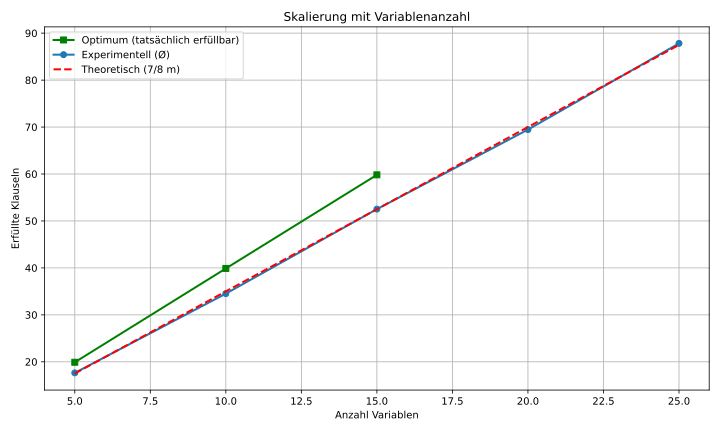
\includegraphics[width=0.95\textwidth]{experiment-results.pdf}
	\caption{Experimentelle Ergebnisse des 3-KNF Algorithmus mit Zufall}
	\label{fig:experiments}
\end{figure}
Beobachtbar ist, dass die Anzahl der erfüllten Klauseln durch den 3-KNF Algorithmus mit Zufall der theoretischen erwarteten Anzahl erfüllter Klauseln entspricht. Bis zu einer Anzahl von 15 Variablen ist die Anzahl der erfüllten Klauseln durch den 3-KNF Algorithmus mit Zufall nicht so hoch wie die optimale, d.h. maximale, Anzahl erfüllbarer Klauseln.

\section{Wahrscheinlichkeitsverteilungen}

Wann immer die Lehre vom Zufall in der Mathematik so verlassen wird, dass sie in der Praxis nicht mehr anwendbar ist, verletzen wir das eigentliche Ziel der Mathematik in diesem wichtigen Thema. Beim Erwartungswert war dies schon der Fall, denn auf die Augenzahl 3,5 wird der Würfel nie zufällig fallen. Damit muss die Lehre vom Zufall in der Mathematik sehr vorsichtig entwickelt werden. Denn wenn man zum Beispiel den Versuch einen Würfel zu würfeln oft wiederholt, ist beobachtbar, dass die Abweichung vom Erwartungswert beachtlich ist.

Die bekannten Wahrscheinlichkeitsverteilungen der Mathematik sind für die unterschiedlichen Versuche mit diskreten Ereignissen mit großer Genauigkeit und Vorsicht anzuwenden. Wird ein Versuch in seiner Beschreibung auf eine Anwendung einer Wahrscheinlichkeitsverteilung überprüft, können kleinste Details in der Beschreibung des Versuchs entscheidend sein für die Wahl der Wahrscheinlichkeitsverteilungen. Wird ein Detail in der Beschreibung des Versuchs übersehen und eine andere Wahrscheinlichkeitsverteilung gewählt, kann dies in der Analyse für den Versuch zu einem anderen Ergebnis führen.

Im Folgenden werden die unterschiedlichen Wahrscheinlichkeitsverteilungen aufgeführt. Dabei sollen Gemeinsamkeiten auffallen und dahin führen, dass sie diese Verteilungen mit Genauigkeit und Vorsicht anzuwenden sind.

\subsection{Bernoulli-Verteilung}

Die Bernoulli-Verteilung beschreibt Versuche, bei denen es nur zwei mögliche Ereignisse gibt. Ein Ereignis wird als Erfolg bezeichnet und das andere als Misserfolg. Zum Beispiel kann beim Wurf einer Münze das Ereignis Kopf als Erfolg und das Ereignis Zahl als Misserfolg bezeichnet werden. Ebenso kann beim Würfeln eines Würfels das Ereignis, dass der Würfel auf die Augenzahl $6$ fällt, als Erfolg bezeichnet werden und alle anderen Ereignisse, dass der Würfel auf die Augenzahlen $1, 2, 3, 4$ oder $5$ fällt, als Misserfolg.

Für einen Versuch, der durch die Bernoulli-Verteilung beschrieben wird, wird eine Zufallsvariable $X$ definiert durch
\begin{align}
	X = 
	\begin{cases} 
		1, & \text{falls Erfolg eintritt} \\
		0, & \text{falls Misserfolg eintritt}
	\end{cases}
\end{align}
Die Wahrscheinlichkeit für den Erfolg wird mit $p$ bezeichnet, also $P(X = 1) = p$. Die Wahrscheinlichkeit für den Misserfolg ist dann $P(X = 0) = 1 - p$. Es ist wichtig zu beachten, dass die Summe aller Wahrscheinlichkeiten $p + (1-p) = 1$ ergibt. Damit ist der Versuch mathematisch vollständig beschrieben.

Der Erwartungswert einer bernoulli-verteilten Zufallsvariable $X$ berechnet sich wie folgt:
\begin{align}
	E[X] &= 1 \cdot P(X = 1) + 0 \cdot P(X = 0) \\
	&= 1 \cdot p + 0 \cdot (1-p) \\
	&= p.
\end{align}
Das bedeutet, bei einem Versuch, der durch die Bernoulli-Verteilung beschrieben wird, erwarten wir im Mittel den Wert $p$. Für den Münzwurf mit $p = \frac{1}{2}$ erwarten wir also den Wert $0{,}5$. Dieser Wert kann nicht eintreten, denn die Münze zeigt entweder Kopf oder Zahl. Der Erwartungswert beschreibt aber formal genau, was bei vielen Wiederholungen dieses Versuchs zu erwarten ist.

\begin{beispiel}
	Ein Basketballspieler trifft den Korb mit einer Wahrscheinlichkeit von $p = 0{,}7$. Bei einem einzelnen Wurf wird der Erfolg (Treffer) mit der Zufallsvariable $X$ beschrieben, die bernoulli-verteilt ist mit Parameter $p = 0{,}7$. Der erwartete Wert ist $E[X] = 0{,}7$.
\end{beispiel}

Die Bernoulli-Verteilung ist die einfachste aller Wahrscheinlichkeitsverteilungen. Sie ist die Grundlage für viele weitere Verteilungen. Wird ein Versuch, der durch die Bernoulli-Verteilung beschrieben wird, mehrfach unabhängig wiederholt, ergeben sich andere Wahrscheinlichkeitsverteilungen, die auf der Bernoulli-Verteilung aufbauen.

\subsection{Geometrische Verteilung}

Die geometrische Verteilung beschreibt Versuche, bei denen ein Bernoulli-Versuch so oft wiederholt wird, bis zum ersten Mal ein Erfolg eintritt. Es stellt sich die Frage: Wie viele Versuche sind nötig, bis der erste Erfolg eintritt? Beim Würfeln eines Würfels kann man fragen: Wie oft muss der Würfel geworfen werden, bis zum ersten Mal die Augenzahl $6$ fällt? Bei diesem Versuch wird der Würfel so lange geworfen, bis die Augenzahl $6$ das erste Mal erscheint.

Für einen Versuch, der durch die geometrische Verteilung beschrieben wird, wird eine Zufallsvariable $X$ definiert durch
\begin{align}
	X = \{\text{Anzahl der Versuche bis zum ersten Erfolg}\}.
\end{align}
Die Wahrscheinlichkeit, dass der erste Erfolg genau beim $k$-ten Versuch eintritt, berechnet sich wie folgt. Es müssen zunächst $k-1$ Misserfolge eintreten, jeder mit Wahrscheinlichkeit $1-p$, und dann muss beim $k$-ten Versuch ein Erfolg mit Wahrscheinlichkeit $p$ eintreten. Damit ergibt sich:
\begin{align}
	P(X = k) = (1-p)^{k-1} \cdot p, \quad k = 1, 2, 3, \ldots
\end{align}
Es ist wichtig zu überprüfen, dass die Summe aller Wahrscheinlichkeiten $1$ ergibt. Dies ist tatsächlich der Fall, denn es gilt:
\begin{align}
	\sum_{k=1}^{\infty} P(X = k) = \sum_{k=1}^{\infty} (1-p)^{k-1} \cdot p = p \cdot \frac{1}{1-(1-p)} = p \cdot \frac{1}{p} = 1.
\end{align}
Damit ist der Versuch mathematisch vollständig beschrieben.

Der Erwartungswert einer geometrisch verteilten Zufallsvariable $X$ beträgt:
\begin{align}
	E[X] = \frac{1}{p}.
\end{align}
Das bedeutet, im Erwartungswert benötigen wir $\frac{1}{p}$ Versuche bis zum ersten Erfolg. Für das Würfeln einer $6$ mit einem Würfel ist $p = \frac{1}{6}$. Damit erwarten wir $E[X] = \frac{1}{1/6} = 6$ Würfe bis zum ersten Mal die Augenzahl $6$ fällt. Dies ist ein intuitives Ergebnis. Wird der Versuch in der Praxis durchgeführt, kann es sein, dass die $6$ bereits beim ersten Wurf fällt. Es kann aber auch sein, dass die $6$ erst nach 20 Würfen das erste Mal fällt. Der Erwartungswert beschreibt das, was im Mittel über viele Wiederholungen dieses gesamten Versuchs zu erwarten ist.

\begin{beispiel}
	Ein Unternehmen ruft potenzielle Kunden an. Jeder Kunde kauft mit Wahrscheinlichkeit $p = 0{,}2$ das Produkt. Die Anzahl der Anrufe bis zum ersten Verkauf ist geometrisch verteilt mit Parameter $p = 0{,}2$. Im Erwartungswert sind $E[X] = \frac{1}{0{,}2} = 5$ Anrufe nötig bis zum ersten Verkauf.
\end{beispiel}

Die geometrische Verteilung zeigt, wie vorsichtig der Erwartungswert interpretiert werden muss. In der Praxis kann die tatsächliche Anzahl der benötigten Versuche erheblich vom Erwartungswert abweichen. Dies ist bei allen Wahrscheinlichkeitsverteilungen zu beachten.

\subsection{Gaußsche Verteilung}

Die Gaußsche Verteilung, auch Normalverteilung genannt, beschreibt kontinuierliche Ereignisse. Bis jetzt wurden nur diskrete Ereignisse betrachtet. Bei kontinuierlichen Ereignissen kann die Zufallsvariable jeden beliebigen Wert aus einem Intervall annehmen, zum Beispiel alle reellen Zahlen. Die Gaußsche Verteilung ist die wichtigste Verteilung für kontinuierliche Ereignisse in der Praxis.

Ein Beispiel für einen Versuch mit kontinuierlichen Ereignissen ist die Messung der Körpergröße von Menschen. Die Körpergröße kann jeden Wert aus einem bestimmten Intervall annehmen, zum Beispiel zwischen $150$ cm und $210$ cm. Die Körpergröße ist damit keine diskrete Größe wie die Augenzahl beim Würfeln, sondern eine kontinuierliche Größe.

Für einen Versuch, der durch die Gaußsche Verteilung beschrieben wird, wird eine Zufallsvariable $X$ definiert, die Werte aus den reellen Zahlen annehmen kann. Die Gaußsche Verteilung wird durch zwei Parameter beschrieben: den Erwartungswert $\mu$ und die Varianz $\sigma^2$. Der Erwartungswert $\mu$ gibt an, um welchen Wert herum die Zufallsvariable streut. Die Varianz $\sigma^2$ gibt an, wie stark die Zufallsvariable um den Erwartungswert streut. Die Standardabweichung $\sigma$ ist die Wurzel aus der Varianz. Die Wahrscheinlichkeitsdichte der Gaußschen Verteilung ist gegeben durch:
\begin{align}
	f(x) = \frac{1}{\sqrt{2\pi\sigma^2}} \cdot e^{-\frac{(x-\mu)^2}{2\sigma^2}}.
\end{align}
Abbildung \ref{fig:gauss-dist} zeigt die Gaußsche Verteilung.
\begin{figure}[htbp]
	\centering
	\includegraphics[width=0.85\textwidth]{gauss-dist.pdf}
	\caption{Gaußsche Verteilung}
	\label{fig:gauss-dist}
\end{figure}
Bei kontinuierlichen Verteilungen kann nicht mehr nach der Wahrscheinlichkeit für ein einzelnes Ereignis gefragt werden, denn diese ist immer $0$. Stattdessen wird nach der Wahrscheinlichkeit gefragt, dass die Zufallsvariable $X$ in einem bestimmten Intervall $[a, b]$ liegt. Diese Wahrscheinlichkeit berechnet sich durch das Integral:
\begin{align}
	P(a \le X \le b) = \int_a^b f(x) \, dx.
\end{align}
Es ist wichtig zu überprüfen, dass das Integral über alle möglichen Werte $1$ ergibt. Dies ist tatsächlich der Fall, denn es gilt:
\begin{align}
	\int_{-\infty}^{\infty} f(x) \, dx = 1.
\end{align}
Damit ist die Gaußsche Verteilung mathematisch vollständig beschrieben.

\begin{beispiel}
	Die Körpergröße von erwachsenen Männern in Deutschland ist annähernd normalverteilt mit Erwartungswert $\mu = 180$ cm und Standardabweichung $\sigma = 7$ cm. Die Wahrscheinlichkeit, dass ein zufällig ausgewählter Mann eine Körpergröße zwischen $173$ cm und $187$ cm hat, entspricht etwa $68\%$. Dies ist ein bekanntes Ergebnis der Gaußschen Verteilung: Etwa $68\%$ aller Werte liegen im Intervall $[\mu - \sigma, \mu + \sigma]$.
\end{beispiel}

Die Gaußsche Verteilung hat eine besondere Eigenschaft: Viele Größen in der Natur und in der Praxis sind annähernd normalverteilt. Dies liegt daran, dass die Gaußsche Verteilung oft entsteht, wenn viele unabhängige Zufallseinflüsse zusammenwirken. Dieser Zusammenhang wird durch den Zentralen Grenzwertsatz der Mathematik beschrieben.

Nicht jede Größe ist normalverteilt. Wird eine Größe fälschlicherweise als normalverteilt angenommen, können die Ergebnisse der Analyse völlig falsch sein. Zum Beispiel sind Aktienkurse nicht normalverteilt, obwohl dies oft angenommen wird. Extreme Ereignisse, sogenannte Ausreißer, treten bei Aktienkursen viel häufiger auf als die Gaußsche Verteilung vorhersagt. Dies kann zu erheblichen Fehleinschätzungen führen.

Die Gaußsche Verteilung ist ein mächtiges Werkzeug, aber sie muss mit Genauigkeit und Vorsicht angewendet werden. Nur wenn die Voraussetzungen für ihre Anwendung erfüllt sind, liefert sie zuverlässige Ergebnisse.

\subsection{Anwendung: Hybrider Registerspeicher}

Die Gaußsche Verteilung findet nicht nur in der Statistik Anwendung, sondern auch in der Informatik und im Hardware-Design. Ein interessantes Beispiel ist die Optimierung von Registerspeichern in Prozessoren. Dabei wird beobachtet, dass die Zugriffe auf Register nicht gleichmäßig verteilt sind, sondern einer Gaußschen Verteilung folgen. Einige Register werden sehr häufig verwendet, während andere Register selten genutzt werden.

Anstatt alle Register gleich zu behandeln, kann man eine hierarchische Struktur einführen. Die Register, die am häufigsten genutzt werden, werden in schnellem und teurem Speicher realisiert. Die Register, die seltener genutzt werden, werden in langsamem und günstigem Speicher realisiert. Für diesen Versuch wird eine Zufallsvariable $X$ definiert durch
\begin{align}
	X = \{\text{Register-Index, auf den zugegriffen wird}\}.
\end{align}
Die Beobachtung zeigt, dass $X$ annähernd normalverteilt ist mit einem Erwartungswert $\mu$ und einer Standardabweichung $\sigma$. Der Erwartungswert $\mu$ gibt an, welcher Register-Index im Mittel am häufigsten genutzt wird. Die Standardabweichung $\sigma$ gibt an, wie stark die Zugriffe um diesen Erwartungswert streuen.

Der hierarchische Aufbau des Registerspeichers erfolgt in zwei Bereichen. Der erste Bereich, genannt Tier 1, enthält etwa 32 bis 64 Register. Diese Register liegen nahe beim Erwartungswert $\mu$ der Verteilung, also im Intervall $[\mu - \sigma, \mu + \sigma]$. Wie bei der Körpergröße im vorherigen Beispiel wissen wir, dass etwa $68\%$ aller Zugriffe auf Register in diesem Intervall liegen. Diese Register werden in schnellem Speicher realisiert. Der zweite Bereich, genannt Tier 2, enthält alle anderen Register. Diese Register werden in langsamem, aber günstigem Speicher realisiert.

Um zu ermitteln, welche Register zu Tier 1 gehören, muss das Zugriffsmuster analysiert werden. Dafür wird während des Betriebs gezählt, wie oft auf jedes Register zugegriffen wird. Diese Zählung ist ein Versuch mit diskreten Ereignissen. Für jedes Register $i$ wird eine Zufallsvariable $Y_i$ definiert durch
\begin{align}
	Y_i = \{\text{Anzahl der Zugriffe auf Register } i\}.
\end{align}
Nach einer gewissen Laufzeit kann aus den Werten von $Y_i$ die Verteilung der Zugriffe ermittelt werden. Die Register mit den höchsten Werten von $Y_i$ werden zu Tier 1 zugeordnet.

Es ist wichtig zu beachten, dass die Zugriffsmuster sich während der Laufzeit ändern können. Ein Programm kann zunächst häufig auf bestimmte Register zugreifen und später auf andere Register. Der Erwartungswert $\mu$ und die Standardabweichung $\sigma$ der Verteilung können sich also verschieben. Damit ist die Zuordnung der Register zu den Bereichen Tier 1 und Tier 2 nicht statisch, sondern muss dynamisch angepasst werden. Dies ist ein wichtiges Detail, das bei der Implementierung beachtet werden muss. Die mathematische Beschreibung mit der Gaußschen Verteilung bleibt dabei vollständig -- es ändert sich nur, welche Register gerade im Intervall $[\mu - \sigma, \mu + \sigma]$ liegen.

Die Kostenersparnis durch diesen Ansatz lässt sich berechnen. Sei $n_1$ die Anzahl der Register in Tier 1 und $n_2$ die Anzahl der Register in Tier 2. Sei $c_1$ der Preis pro Register in Tier 1 und $c_2$ der Preis pro Register in Tier 2, wobei $c_1 \gg c_2$ gilt. Die Gesamtkosten betragen
\begin{align}
	C = n_1 \cdot c_1 + n_2 \cdot c_2.
\end{align}
Ohne die hierarchische Struktur wären alle $n_1 + n_2$ Register in teurem Speicher realisiert, mit Gesamtkosten von $(n_1 + n_2) \cdot c_1$. Die Kostenersparnis beträgt damit
\begin{align}
	\Delta C = (n_1 + n_2) \cdot c_1 - (n_1 \cdot c_1 + n_2 \cdot c_2) = n_2 \cdot (c_1 - c_2).
\end{align}
Da typischerweise $n_2 \gg n_1$ gilt, ist die Kostenersparnis erheblich.

Dieses Beispiel zeigt, wie die Gaußsche Verteilung in der Praxis angewendet werden kann. Es zeigt auch, wie wichtig es ist, die Voraussetzungen zu überprüfen. Die Annahme, dass die Zugriffe auf Register normalverteilt sind, muss im Detail überprüft werden. Besteht ein anderes Zugriffsmuster, kann die hierarchische Struktur ineffizient sein.

\section{Zusammenfassung}

In diesem Dokument wurde die Lehre vom Zufall in der Mathematik entwickelt. Ausgangspunkt war das einfache Beispiel des Würfelns eines Würfels. An diesem Beispiel wurden die grundlegenden Begriffe eingeführt: der Versuch, die Ereignisse, die Menge aller Ereignisse $\Omega$, und die Wahrscheinlichkeit für den Zufall eines Ereignisses. Es wurde gezeigt, dass ein Versuch mathematisch vollständig beschrieben ist, wenn die Summe aller Wahrscheinlichkeiten der Zufälle aller Ereignisse insgesamt $1$ ergibt.

Für die Analyse von Versuchen wurde das Konzept der Zufallsvariable eingeführt. Eine Zufallsvariable beschreibt den Zufall für das Ereignis variabel für den konkreten Ausgang. Mit Hilfe der Zufallsvariable kann der Erwartungswert berechnet werden. Der Erwartungswert beschreibt formal am genauesten, welcher Ausgang bei einem Versuch zu erwarten ist. Es wurde aber auch gewarnt, dass der Erwartungswert in der Praxis nicht immer sinnvoll interpretierbar ist. Beim Würfeln eines Würfels ergibt sich ein Erwartungswert von $3{,}5$, eine Augenzahl, die es nicht gibt. Der Erwartungswert beschreibt das, was im Mittel über viele Wiederholungen des Versuchs zu erwarten ist.

Am Beispiel des 3-KNF Algorithmus wurde gezeigt, wie Zufall in der Informatik eingesetzt wird, um effiziente Algorithmen zu entwickeln. Der Algorithmus mit Zufall für 3-KNF erreicht eine Approximationsgüte von $\frac{7}{8}$. Das bedeutet, dass im Erwartungswert mindestens $87{,}5\%$ aller erfüllbaren Klauseln erfüllt werden. Die experimentellen Ergebnisse zeigen, dass die theoretische Analyse mit der Praxis übereinstimmt. Dies ist ein Beispiel dafür, dass die mathematische Beschreibung des Zufalls in der Praxis anwendbar ist und zu verlässlichen Ergebnissen führt.

Die Wahrscheinlichkeitsverteilungen sind zentrale Werkzeuge für die Analyse von Versuchen mit Zufall. Es wurden drei Verteilungen vorgestellt: die Bernoulli-Verteilung für Versuche mit zwei möglichen Ereignissen, die geometrische Verteilung für die Anzahl der Versuche bis zum ersten Erfolg, und die Gaußsche Verteilung für kontinuierliche Ereignisse. Jede dieser Verteilungen hat ihre spezifischen Anwendungsbereiche. Es wurde mehrfach betont, dass die Wahl der richtigen Verteilung entscheidend ist. Kleinste Details in der Beschreibung des Versuchs können darüber entscheiden, welche Verteilung anwendbar ist. Wird eine andere Verteilung gewählt, führt dies zu anderen Ergebnissen in der Analyse.

Am Beispiel des hybriden Registerspeichers wurde eine konkrete Anwendung der Gaußschen Verteilung in der Hardware-Entwicklung gezeigt. Die Beobachtung, dass Zugriffe auf Prozessorregister annähernd normalverteilt sind, ermöglicht den Aufbau einer hierarchischen Speicherarchitektur. Register im Zentrum der Verteilung werden in schnellem, teurem Speicher realisiert, während selten genutzte Register in langsamem, günstigem Speicher untergebracht werden. Die Kostenersparnis ist erheblich, da typischerweise nur etwa 10 bis 15 Prozent der Register in teurer Technologie gefertigt werden müssen. Dieses Beispiel zeigt, wie die mathematische Beschreibung des Zufalls zu praktischen Verbesserungen in der Informationsverarbeitung führen kann.

Die Lehre vom Zufall in der Mathematik muss mit Genauigkeit und Vorsicht entwickelt und angewendet werden. Wann immer die mathematische Beschreibung so weit von der Praxis entfernt ist, dass sie nicht mehr anwendbar ist, wird das eigentliche Ziel der Mathematik in diesem Thema verletzt. Die Mathematik soll helfen, den Zufall zu verstehen und in der Praxis verlässliche Entscheidungen zu treffen.

\subsection{Ausblick}

Die in diesem Dokument vorgestellten Konzepte bilden die Grundlage für weiterführende Themen in der Wahrscheinlichkeitstheorie und Statistik. Es gibt viele weitere Wahrscheinlichkeitsverteilungen, die für spezifische Anwendungen entwickelt wurden. Die Binomialverteilung beschreibt die Anzahl der Erfolge bei mehrfacher Wiederholung eines Bernoulli-Versuchs. Die Poisson-Verteilung beschreibt die Anzahl von Ereignissen, die in einem festen Zeitintervall eintreten. Die Exponentialverteilung beschreibt die Wartezeit bis zum nächsten Ereignis. Jede dieser Verteilungen hat ihre eigenen Eigenschaften und Anwendungsbereiche, die sorgfältig studiert werden müssen.

Der Zentrale Grenzwertsatz ist ein fundamentales Ergebnis der Wahrscheinlichkeitstheorie. Er besagt, dass die Summe vieler unabhängiger Zufallsvariablen annähernd normalverteilt ist, unabhängig davon, welche Verteilung die einzelnen Zufallsvariablen haben. Dies erklärt, warum die Gaußsche Verteilung in der Natur und in der Praxis so häufig auftritt. Der Zentrale Grenzwertsatz ist die theoretische Grundlage für viele statistische Verfahren.

In der Statistik werden die Konzepte der Wahrscheinlichkeitstheorie verwendet, um aus Beobachtungen Schlüsse zu ziehen. Wenn wir einen Würfel mehrmals werfen und die Ergebnisse beobachten, können wir mit statistischen Methoden überprüfen, ob der Würfel fair ist. Wenn wir die Körpergröße von Menschen messen, können wir mit statistischen Methoden Rückschlüsse auf die Parameter der Verteilung ziehen. Die Statistik verbindet die theoretische Wahrscheinlichkeitsrechnung mit der praktischen Datenanalyse.

Der Einsatz von Zufall in Algorithmen, wie beim 3-KNF Algorithmus gezeigt, ist ein aktives Forschungsgebiet in der Informatik. Randomisierte Algorithmen können oft effizienter sein als deterministische Algorithmen. Sie werden in vielen Bereichen eingesetzt, von der Kryptographie über die Optimierung bis hin zum maschinellen Lernen. Das Verständnis der wahrscheinlichkeitstheoretischen Grundlagen ist essentiell, um solche Algorithmen zu entwickeln und zu analysieren.

Die Anwendung der Gaußschen Verteilung auf Hardware-Architekturen eröffnet weitere Forschungsmöglichkeiten. Dies wurde beim hybriden Registerspeicher gezeigt. Ähnliche Ansätze können auf Cache-Hierarchien, Speicherverwaltung und Netzwerkarchitekturen übertragen werden. Überall dort, wo Zugriffsmuster beobachtbar sind und einer statistischen Verteilung folgen, kann durch geschickte Ausnutzung dieser Verteilung eine Optimierung erreicht werden. Die Herausforderung liegt dabei darin, die Annahmen über die Verteilung zu überprüfen und die Systeme so zu gestalten, dass sie sich an veränderte Muster anpassen können. Künstliche Intelligenz kann dabei helfen, die Parameter der Verteilungen kontinuierlich zu lernen und die Architektur entsprechend anzupassen.

Die Lehre vom Zufall in der Mathematik ist ein hilfreiches und vielversprechendes Gebiet gerade für die Entwicklung von Algorithmen. Sie verbindet mathematische Beschreibungen mit praktischen Anwendungen und kann dabei helfen, Probleme effizienter zu lösen.
	
\end{document}